\chapter{SEGURANÇA DE REDE}
\label{cap:seguranca}

    Estar conectado à internet requer cuidados, pois dispositivos expostos à rede pública estão sujeitos às ameças de segurança que podem atacá-los. Sistema completamente seguro não existe, mas usuários finais devem tomar os devidos cuidados em suas redes locais bem como os ISPs também devem tomar as medidas que estiverem ao alcance. No ISP, as competências de segurança atribuídas ao NOC são manter seguros os serviços, protocolos e as redes de telecomunicações, que estão nos níveis mais baixos da implementação das políticas de segurança da informação, enquanto o desenvolvimento de software e interação humano-computador estão em alto nível. A segurança é um acordo que deve ser cumprido por todas as partes em todos os níveis para minimização dos incidentes.

\section{IP Blacklist}

    A Minasnet, como sendo um AS, tem delegação sobre vários blocos de endereços IP que dão aos seus assinantes identidade na internet. O primeiro problema quanto à segurança surge neste ponto, pois a conectividade traz riscos, que se iniciam pelo IP público através do qual os ataques conseguem propagar-se pela internet (ou pela intranet, via rede privada).
    
    Grande parte dos \textit{worms} são propagados pela internet através de \textit{spam}, que são enviados de maneira massiva por dispositivos infectados, sejam computadores, smartphones, roteadores domésticos e até roteadores de \textit{core}, basta ter conexão à internet que se torna vulnerável a \textit{botnets}. 
    
    Uma forma de controlar o envio de spam, por parte dos provedores de serviço, é a utilização de listas negras com IPs que foram identificados como fonte de envio de \textit{spam}. Chamadas de \textit{Real-time Blackhole List} (RBL), doravante \textit{blacklist}, proporcionam a listagem de IPs detectados recentemente como participantes ativos de \textit{botnet} para envio de \textit{spam}, possibilitando ao provedor de serviço bloquear todo o tráfego de e-mail a partir daquele endereço IP listado. 
    
    Neste trabalho, foi feito uso de RBL com a finalidade de monitoramento de IPs do AS que estão listados na blacklist, afim de identificar infecções no núcleo da rede (devido às vulnerabilidades associadas a equipamentos MikroTik com IP público), bem como nos assinantes. Para isso, foi utilizado o \textit{Composite Blocking List} (CBL)\footnote{CBL \url{https://www.abuseat.org} é uma divisão da Spamhaus.}, uma RBL com consulta no padrão DNS Blacklist (DNSBL).
    
    DNSBL é especificado pela RFC 5782, funcionando com estrutura semelhante a um DNS reverso. Cada IP listado em uma DNSBL tem um subdomínio correspondente, sendo que cada entrada de subdomínio é criada revertendo os octetos do IP e concatenando com o domínio da DNSBL. Uma consulta à DNSBL retorna no registro {\tt A} o endereço 127.0.0.2 e no registro {\tt TXT} a descrição do motivo pelo qual o IP está listado na \textit{blacklist} \cite{rfc5782}. Quando o IP não está na \textit{blacklist}, a consulta retorna o erro {\tt NXDOMAIN}. Por exemplo, uma consulta para verificar se o IP 192.0.2.99 está listado na CBL seria feita a partir da entrada 99.2.0.192.cbl.abuseat.org e, em caso de listagem positiva, o link informado no registro {\tt TXT} daria um relatório detalhado da origem e qual tipo de infecção foi detectada atrás desse IP. Em terminal de comando Linux, a consulta pode ser feita da seguinte forma, para os registros {\tt A} e {\tt TXT}, respectivamente, conforme Figura \ref{fig:dnsbl_query}.
    
    \begin{figure}[!htb]
        \centering
        \caption{Exemplo de consulta à DNSBL CBL via terminal Linux.} 
        \label{fig:dnsbl_query}
        
        \begin{Verbatim}[fontsize=\normalsize]
            host -t A 99.2.0.192.cbl.abuseat.org
            host -t TXT 99.2.0.192.cbl.abuseat.org
        \end{Verbatim} 

        {\small Fonte: do autor (2020).} 
    \end{figure}
    
    O monitoramento foi feito de maneira automatizada, através de um simples programa feito em Python para fazer a varredura de todos os blocos de IP do AS, que até o momento é constituído por 8.192 endereços. O programa varre todos os endereços e retorna um resumo contendo somente aqueles que estão listados na \textit{blacklist}, que serão analisados através do relatório detalhado na página da CBL.
    
    O Gráfico \ref{fig:plot_blacklist} mostra o resultado do monitoramento de IPs da Minasnet listados na CBL entre abril e setembro de 2019 e o Anexo A é um exemplo de relatório detalhado fornecido pela plataforma, contendo informações de origem, destino e tipo de infecção, além de sugestões para correção do problema. Apesar de o Gráfico \ref{fig:plot_blacklist} apresentar subidas e descidas acentuadas na contagem dos IPs listados na \textit{blacklist}, não foi evidenciada nenhuma relação imediata entre a quantidade de IPs listados com as tratativas implementadas em firewall para tentar mitigar o problema, o que caracteriza que o \textit{spam} está originando-se na rede interna dos assinantes e trafegando na internet pela camada de aplicação, como pode ser visto no relatório apresentado no Anexo A, que relata a detecção através de tráfego HTTP.
    
    \begin{grafico}[!htb]
        \centering
        \caption{Contagem de IPs do AS listados na CBL entre abril e setembro de 2019.} 
        \label{fig:plot_blacklist} 
        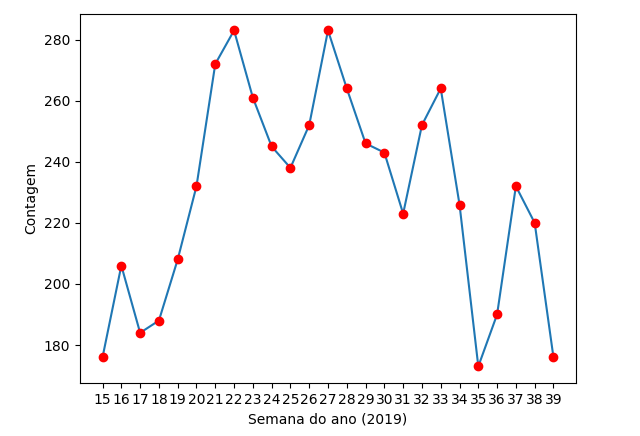
\includegraphics[scale=0.5]{img/plot_blacklist.png} \\
        {\small Fonte: do autor (2020).} 
    \end{grafico}
    
    As informações sobre os endereços IP listados na CBL são detectadas por \textit{honeypots}. Os \textit{Honeypots} são máquinas que emulam determinados sistemas operacionais e serviços, para que um atacante interaja com ela sem que perceba que está entrando em uma armadilha \cite{spampots2007}. É utilizando este artifício que a CBL faz a detecção de \textit{botnets} e registra o IP de origem do \textit{spam}. A Figura \ref{fig:honeypot} mostra um exemplo de arquitetura utilizada para essa detecção. A descrição da metodologia utilizada pela plataforma pode ser obtida (em inglês) no site da CBL. 
    
    \begin{figure}[!htb]
        \centering
        \caption{Arquitetura de um honeypot para detecção de spam.} 
        \label{fig:honeypot} 
        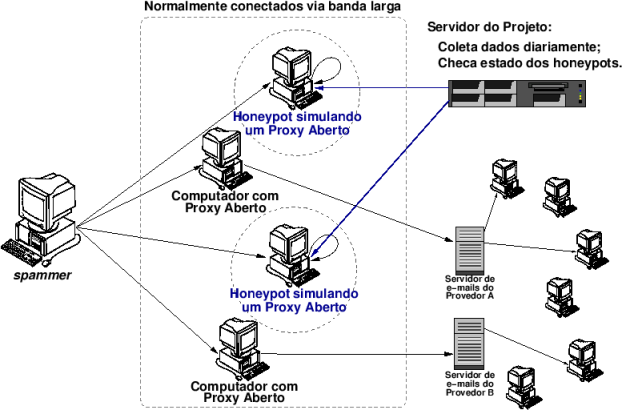
\includegraphics[scale=0.8]{img/honeypot.png} \\
        {\small Fonte: CERT (2007).} 
    \end{figure}
    
    A CBL oferece a opção de remoção manual de um IP listado, porém essa ação não soluciona o problema de fato, uma vez que caso a infecção persista, muito provavelmente o IP retornará à listagem. Por isso, a melhor solução para o problema da \textit{blacklist} é a correção efetiva de vulnerabilidades existentes na rede, sendo que após um período de 28 dias sem nenhuma ocorrência, automaticamente o IP é removido da lista.

\section{Vulnerabilidades de rede}

    O CERT.br (Centro de Estudos, Resposta e Tratamento de Incidentes de Segurança no Brasil) é responsável por tratar incidentes de segurança computacional envolvendo redes conectadas à internet brasileira. Por isso, possui rotina de analisar, por amostragem, IPs registrados pelo Registro.br e notificar os responsáveis pelo AS no qual foi detectada alguma vulnerabilidade.
    
    Vulnerabilidades de rede podem ser exploradas através de portas abertas em dispositivos. Portas abertas de serviços mal configurados são fonte para ataques de invasão, envio de \textit{spam} e DDoS (negação de serviço).
    
    Dessa forma, o CERT.br faz, regularmente, amostragem de IPs dos ASs brasileiros para realizar varredura de portas abertas, filtrando portas de serviços específicos que possam ser explorados por atacantes na internet e notificando as operadoras responsáveis. Uma varredura de portas, ou \textit{scan} de portas, pode ser feita a partir de terminal de comando pela ferramenta {\tt nmap}. Através do comando apresentado na Figura \ref{fig:nmap}, pode ser feita a varredura de todas as portas do \textit{host} 192.0.2.99, por exemplo. Os parâmetros {\tt -sU} e {\tt -sT} especificam a utilização de portas UDP e TCP na varredura, respectivamente, {\tt -p-} é um \textit{alias} para {\tt -p0-65535}, que faz varredura de todas as portas possíveis e {\tt -T5} é utilizado para uma execução mais rápida.

    \begin{figure}[!htb]
        \centering
        \caption{Exemplo de uso do nmap para varredura completa de portas.} 
        \label{fig:nmap} 
        
        \begin{Verbatim}[fontsize=\normalsize]
            nmap -sU -sT -p- 192.0.2.99 -T5
        \end{Verbatim} 
        
        {\small Fonte: do autor (2020).} 
    \end{figure}
    
    Quando portas de serviços vulneráveis são detectadas como abertas, o CERT.br envia um e-mail contendo relatório detalhado da vulnerabilidade ao responsável pela administração daquele IP escaneado, além de fornecer sugestões para correção do problema. O Anexo B é um e-mail enviado pelo CERT.br à Minasnet após detectar vulnerabilidade no protocolo SOCKS em dispositivos MikroTik na rede.
    
    A maioria das vulnerabilidades surgem devido a configuração errônea de CPEs por parte dos instaladores nas residências ou nos estabelecimentos comerciais, ou por parte dos analistas de rede na configuração de roteadores do núcleo da rede. A correção dessas vulnerabilidades pode ser resolvida com a configuração correta de todos os equipamentos, o que é uma meta difícil de ser atingida, devido ao fator humano ser responsável pela garantia das configurações. Assim, quanto menor a dependência de fatores humanos, melhor a abordagem de tratamento de vulnerabilidades. Neste trabalho, foi utilizada a abordagem de firewall para filtragem de portas e VPN para controlar o acesso. 
    
        % quanto menor a dependência de fatores humanos, melhor a solução de tratamento de vulnerabilidades. Neste trabalho, foi utilizada a abordagem ...
    
    
    
    As principais vulnerabilidades exploradas por atacantes que foram tratadas através do firewall implementado são os ataques por obtenção de informações, por invasão e por negação de serviço, que geralmente estão nas notificações do CERT.br por serem recorrentes.

\section{Implantação de VPN}

    A abordagem utilizada no trabalho foi, primeiro, controlar o acesso remoto implementando um serviço de autenticação através de VPN e, depois, fazer a filtragem de portas. Para controle de acesso, foi adotado o OpenVPN\footnote{OpenVPN \url{https://openvpn.net} é uma VPN SSL open source.}, uma solução gratuita, customizável e portável para várias plataformas. OpenVPN é um serviço completo de VPN SSL que é executável em um servidor Linux, que pode ser integrado com vários outros serviços e protocolos como for desejável. VPNs L2TP/IPSec e PPTP não possuem tantos recursos e flexibilidade como o OpenVPN suporta. Além disso, OpenVPN é um projeto open source, que conta com uma grande comunidade, com boa documentação e com fórum de suporte e de discussão. OpenVPN também possui serviços prontos para empresas e para usuários finais, a partir do pagamento de assinaturas.
    
    O projeto da VPN é bem simples, possuindo apenas dois requisitos: deve ser instalada em um servidor e possuir autenticação de dois fatores (2FA). Assim, o \textit{deploy} do servidor foi feito em uma VPS (\textit{virtual private server}) Debian Linux, mantida no datacenter da Minasnet, com as seguintes configurações de hardware compartilhadas, pois foi alocada uma máquina virtual para ser o servidor:
    
    \begin{enumerate}[label=\alph*)]
        \item processador: Intel Xeon X7550;
        \item quantidade de núcleos: 2;
        \item memória RAM: 2GB;
        \item disco: 60GB;
        \item capacidade de rede: 1Gbps;
    \end{enumerate}
    
    A configuração do servidor foi feita inicialmente aplicando uma camada básica de segurança, seguindo o princípio do privilégio mínimo, deixando somente as portas necessárias abertas e restringindo o acesso SSH somente ao usuário administrador. Foi elaborado um manual desse procedimento inicial. O manual está disponível para consulta no Apêndice B.
    
    Após aplicado o princípio do privilégio mínimo ao servidor base onde será implantada a VPN, foi feita toda a instalação e configuração do serviço OpenVPN, também foi elaborado manual de todos as configurações efetuadas. O manual completo da implantação do servidor OpenVPN está disponível no Apêndice C.
    
\subsection{Configuração do serviço OpenVPN}
    
    A configuração do servidor OpenVPN consiste em criar uma infraestrutura de chave privada (PKI) utilizando a ferramenta EasyRSA\footnote{EasyRSA \url{https://github.com/OpenVPN/easy-rsa} é um utilitário de CA (\textit{Certification Authority}).}, responsável pela autoridade dos certificados SSL utilizados na VPN. É recomendado manter os servidores de PKI e de VPN em máquinas distintas (serviço de autenticação e de conexão separados), entretanto, para a finalidade deste trabalho, foi mantido um servidor monolítico.
    
    Com a PKI operacional, são feitas as configurações do OpenVPN propriamente ditas, sendo ajustados os parâmetros para funcionamento básico do serviço conforme desejado: permitir que usuários autentiquem-se via internet e acessem a intranet através do túnel criado por essa conexão.
    
    O sistema 2FA utiliza o certificado SSL (mantido pela PKI) e autenticação por usuário e senha (suportada pelo \textit{plugin} PAM do Linux). A vantagem em utilizar PAM é a simplicidade de manutenção das contas de usuários, que é feita utilizando {\tt adduser} para criar um novo usuário, {\tt passwd} para alteração da senha e {\tt deluser} para remoção do usuário do sistema.
    
    Além disso, foi criado um \textit{script} feito em Python para facilitar a criação de chaves e de usuários, ao invés de executar manualmente os comandos do EasyRSA todas as vezes que fossem criados novos usuários. O programa não consiste em uma aplicação CLI totalmente funcional, apenas é um \textit{script} para facilitar a chamada dos comandos de maneira automática, sendo que, em caso de problemas, é demandada experiência em terminal de comando Linux para lidar com erros no EasyRSA, nas contas de usuários ou no gerenciador de serviços {\tt systemd}. É possível construir uma interface mais robusta para gestão da VPN, uma interface web por exemplo, porém está fora do escopo deste trabalho.
    
    Além do servidor OpenVPN de produção, também é mantido um servidor OpenVPN de homologação, que está instalado em outra VPS com PKI distinta, com a finalidade de efetuar testes de funcionalidades sem afetar o ambiente em produção.
    
    O ambiente em produção mantém conexão de dezenas de usuários simultaneamente sem perda de desempenho, servindo de porta de entrada à rede privada do provedor. A configuração atual permite que somente seja possível acessar equipamentos de núcleo da rede através da VPN, restringindo e controlando o acesso remoto a equipamentos críticos somente a usuários autorizados, minimizando a probabilidade de incidência de ataques de invasão nos mesmos.
    
    O servidor OpenVPN principal está na rotina de backup automático dos servidores do datacenter da Minasnet, isso garante tolerância a falhas caso o servidor em produção seja corrompido. Em caso de corrompimento, é necessário somente a restauração de uma imagem do servidor para que não seja perdido nenhum certificado da PKI, deste que o \textit{check-point} esteja em um instante após a inserção do um último usuário. Como a frequência do backup é semanal e não são adicionados novos usuários com tanta frequência, os impactos após uma inconsistência no servidor tendem a ser mínimos.
    
\subsection{Considerações sobre o servidor OpenVPN}

    A manutenção de um servidor OpenVPN demanda perícia em ambiente Linux, pois a resolução de falhas requer análise de log do {\tt systemd}. Um detalhe é que o serviço da VPN não se inicia automaticamente quando o servidor é reiniciado, devido à necessidade de inserção manual do \textit{passphrase} da PKI em prompt no terminal de comandos.
    
    Outro detalhe é que os certificados SSL têm prazo de validade de 3 anos, sendo que não é possível renová-los para estender a data de validade. É importante monitorar a validade dos certificados e gerar novos depois de vencidos para que não haja transtorno para os usuários da VPN.
    
\section{Implementação de firewall}

    Com a VPN operacional, o próximo passo para implementação de segurança na rede é a configuração do sistema de firewall para filtragem de pacotes suspeitos. A finalidade do firewall é mitigar as vulnerabilidades elencadas pelas notificações do CERT.br, bem como garantir a aplicação das políticas de segurança de rede adotadas pelo ISP.
    
    A abordagem de firewall deste trabalho é simples e eficiente, fazendo filtragem por endereços IP e por números de porta, ou seja, o firewall vai inspecionar os cabeçalhos dos pacotes nas camadas de rede e de transporte. Existem modelos de firewall que inspecionam pacotes na camada de aplicação (firewall \textit{layer} 7), porém requerem muito poder de processamento e podem afetar negativamente o \textit{throughput} da rede, sendo dedicados às redes corporativas (universidades e grandes corporações) ao invés de provedores de internet. Filtrar IP e porta é o suficiente para a função do ISP.
    
    Antes da implantação feita neste trabalho, não existia firewall na rede de acesso dos clientes da Minasnet, ou seja, todos os CPEs dos clientes estavam expostos à internet sem nenhum filtro, sendo a única camada de segurança a manutenção de senhas fortes nos equipamentos e configuração correta por parte dos instaladores, algo que nem sempre ocorria. Houve relatos, por exemplo, de antenas Ubiquiti e MikroTik que foram infectadas por \textit{worms} devido às vulnerabilidades nas quais os equipamentos estavam expostos.
    
    Após elencadas as vulnerabilidades às quais os equipamentos da rede são suscetíveis, a tarefa é implementar as regras de firewall para colocá-las em produção em um roteador que faça interface entre os tráfegos de rede, ou seja, que fique intermediando o caminho por onde passarão todos os pacotes. A abordagem deste trabalho utiliza o firewall nativo da plataforma RouterOS dos roteadores MikroTik, que possui seu funcionamento básico semelhante ao iptables do Linux, pois a próprioa plataforma é construída sobre o \textit{kernel} Linux.
    
    Os requisitos de firewall desenvolvidos para a Minasnet, inicialmente, são os seguintes: 
    
    \begin{enumerate}[label=\alph*)]
        \item negar o acesso remoto aos equipamentos primários dos clientes, que desempenham a função de cliente PPPoE;
        \item permitir somente que o NOC e o Help Desk acessem remotamente os equipamentos dos clientes;
        \item permitir que clientes de IP fixo fiquem expostos à internet, sem filtragem por firewall;
        \item negar que clientes acessem a intranet do ISP;
        \item aplicar filtros que corrijam vulnerabilidades detectadas na rede.
    \end{enumerate}
    
\subsection{Regras de firewall no RouterOS}

    O objetivo deste firewall é filtrar conexões de entrada que caracterizem acesso ilegal a equipamentos, conforme regras definidas por IP e porta. Filtrar consiste em descartar pacotes de acordo com as regras.
    
    A topologia utilizada para implantação do firewall aplica as regras diretamente ao concentrador (B-RAS), pois é nele que está a origem (ou destino, dependendo do ponto de vista) do tráfego dos clientes. Colocar outro equipamento intermediando o concentrador com finalidade de firewall não é suficiente, pois não é possível filtrar conexões entre clientes de um mesmo concentrador de acordo com a metodologia utilizada neste trabalho, isso porque a comutação de pacotes é feita em memória neste caso.
    
    De acordo com a documentação do RouterOS \cite{fwmikrotik}, para implementar o firewall de acordo com os requisitos supracitados, são utilizados os seguintes parâmetros oferecidos na tabela \textit{filter} do firewall:
    
    \begin{enumerate}[label=\alph*)]
        \item {\tt address-list}: estrutura de dados do tipo lista contendo endereços que serão alvo das regras, para auxiliar na construção fracamente acoplada dos componentes do firewall;
        \item {\tt action}: ação que o firewall deve executar quando a regra for acionada, como o objetivo é filtrar, será utilizada a ação \textit{drop};
        \item {\tt chain}: caminho que o pacote faz no roteador, como os pacotes que serão filtrados estão sendo roteados, utiliza-se a cadeia \textit{forward};
        \item {\tt protocol}: protocolo de transporte, TCP ou UDP;
        \item {\tt in-interface} ou {\tt out-interface}: interfaces alvos das regras, neste caso, todos os clientes PPPoE;
        \item {\tt src-port} ou {\tt dst-port}: número das portas que serão filtradas pelo firewall.
    \end{enumerate}

    A construção das regras de firewall foram feitas através de \textit{script} nativo para a plataforma. A seguir, estão exemplos da implementação de algumas regras básicas que atendem aos requisitos definidos anteriormente, sendo que, na Figura \ref{fig:firewall_addrlist}, está codificada a primeira etapa da construção do firewall: a definição das listas de IP nas quais as regras de filtragem serão trabalhadas, sendo elas as redes de gerência, que têm acesso privilegiado em toda a rede do ISP, a rede de clientes que contrataram o serviço de IP fixo e desejam ficar expostos à internet, e a rede de Bogons, que neste caso são endereços privados do ISP e não devem ser acessíveis pelos assinantes.
    
    \begin{figure}[!htb]
        \centering
        \caption{Exemplo de criação de address-list para o firewall do RouterOS.} 
        \label{fig:firewall_addrlist}
        
        \begin{Verbatim}[fontsize=\normalsize]
            /ip firewall address-list
            add comment="IP FIXO CLIENTES"                  \
                address=203.0.113.128/25 list=rede_ip_fixo
            add comment="SERVIDOR VPN"                      \
                address=203.0.113.123 list=rede_gerencia
            add comment="HELP DESK"                         \
                address=203.0.113.124 list=rede_gerencia
            add comment="ESCRITORIO NOC"                    \
                address=203.0.113.125 list=rede_gerencia
            add comment="BOGONS"                            \
                address=10.0.0.0/8 list=rede_privada
            add comment="BOGONS"                            \
                address=172.16.0.0/12 list=rede_privada
            add comment="BOGONS"                            \
                address=192.168.0.0/16 list=rede_privada
        \end{Verbatim} 

        {\small Fonte: do autor (2020).} 
    \end{figure}
    
    A utilização de listas de IP não é obrigatória para configuração das regras de firewall, sendo possível inserir cada um dos IPs diretamente. O problema é que a manutenibilidade do firewall fica prejudicada, assim as listas deixam os componentes fracamente conectados e permite que qualquer alteração de IP não necessite de alteração nas regras propriamente ditas, além de deixar o código mais legível, sendo assim uma boa prática na configuração do firewall.
    
    
    
    Um dos primeiros requisitos citados para implementação do firewall foi a necessidade de impedir a invasão aos equipamentos de clientes, permitindo o acesso somente às redes gerenciais da empresa (NOC e Help Desk). O acesso remoto a esses dispositivos é feito através de página web (na maioria dos casos), como também via SSH, Telnet ou Winbox. Assim, na Figura \ref{fig:drop_cpe}, é apresentada a regra que determina o bloqueio de todo acesso externo nas portas de gerência em todos os assinantes, exceto IP fixo, a fim de garantir o cumprimento do requisito de segurança.
    
    \begin{figure}[!htb]
        \centering
        \caption{Regra de firewall para controle de acesso aos CPEs.} 
        \label{fig:drop_cpe}
        
        \begin{Verbatim}[fontsize=\normalsize]
            /ip firewall filter
            add comment="DROP GERENCIA DE CPE"  \
                action=drop                     \
                chain=forward                   \
                out-interface=all-ppp           \
                src-address-list=!rede_gerencia \
                dst-address-list=!rede_ip_fixo  \
                dst-port=0-1023                 \
                protocol=tcp
        \end{Verbatim} 

        {\small Fonte: do autor (2020).} 
    \end{figure}
    
    Outro requisito está codificado na Figura \ref{fig:drop_bogon}, uma regra para impedir a descoberta e o acesso às redes bogons, que são redes privadas. Por serem utilizados IPs privados para endereçar roteadores e servidores do núcleo da rede, é necessário bloquear toda conexão de saída em todos os clientes com destino para a lista de redes privadas (bogons), a fim de garantir o princípio do privilégio mínimo a esses equipamentos. Como se tratam de dispositivos que operam a parte crítica da rede, devem ser acessíveis somente à equipe do NOC, pois se algum hacker conseguir elencar e explorar alguma vulnerabilidade nesses equipamentos, pode causar um prejuízo enorme ao ISP.
    
    \begin{figure}[!htb]
        \centering
        \caption{Regra de firewall para bloqueio de acesso à rede privada do provedor.} 
        \label{fig:drop_bogon}
        
        \begin{Verbatim}[fontsize=\normalsize]
            /ip firewall filter
            add comment="DROP REDE BOGON"     \
                action=drop                   \
                chain=forward                 \
                in-interface=all-ppp          \
                dst-address-list=rede_privada
        \end{Verbatim} 

        {\small Fonte: do autor (2020).} 
    \end{figure}
    
    A Figura \ref{fig:drop_socks} tem a implementação do filtro que impede ataque de \textit{spam} a partir de servidores SOCKS abertos em Mikrotik, bloqueando toda conexão de entrada na porta 4145 TCP em todos os assinantes, sem exceção, por razões de segurança, uma vez que a notificação do CERT.br disponível no Anexo B relata que inclusive clientes de IP fixo estão vulneráveis. Como essa regra foi desenvolvida com a finalidade de corrigir o problema citado no e-mail, todos os assinantes são alvo dessa filtragem.
    
    \begin{figure}[!htb]
        \centering
        \caption{Regra de firewall para correção da vulnerabilidade por SOCKS notificada pelo CERT.br.} 
        \label{fig:drop_socks}
        
        \begin{Verbatim}[fontsize=\normalsize]
            /ip firewall filter
            add comment="DROP SOCKS 4145" \
                action=drop               \
                chain=forward             \
                out-interface=all-ppp     \
                dst-port=4145             \
                protocol=tcp
        \end{Verbatim} 

        {\small Fonte: do autor (2020).} 
    \end{figure}
    
    Não será exposto o script completo de configuração do firewall dos concentradores da Minasnet neste documento, por questão de segurança e de confidencialidade, uma vez que pessoas mal intencionadas poderiam explorar alguma vulnerabilidade que tenha passada despercebida na metodologia utilizada. Mesmo que não exista sistema 100\% seguro, mantendo confidencialidade é possível dificultar o trabalho dos atacantes. Por isso, ficaram descritos aqui somente esses exemplos.
    
\subsection{Considerações sobre o firewall}
    
    A criação de regras de firewall é uma tarefa simples quando se conhece os recursos da plataforma na qual está trabalhando, porém requer cautela, pois configuração errônea pode comprometer a navegação dos assinantes ou então afetar negativamente o processamento dos roteadores nos quais foram feitos a implantação das regras. Devido à familiaridade com iptables, o firewall do RouterOS é intuitivo para quem tem experiência com o sistem Linux, entretanto é um recurso implantado em software. O fato de o firewall não possuir hardware dedicado para a tarefa, limita a capacidade de filtragem que pode ser aplicada através dele.
    
    Após colocar o firewall da Minasnet em produção, notificações recorrentes do CERT.br cessaram. No entanto, novas vulnerabilidades são elencadas frequentemente pelos \textit{scanners} do grupo. Esses eventos determinam a necessidade da contínua tarefa de criação, de melhoria e de aperfeiçoamento das regras do firewall dos concentradores para atender aos novos requisitos de segurança levantados.
    
    A implantação de firewall no concentrador requer cuidado, uma vez que pode comprometer o desempenho da Routerboard. Por isso, foi feito monitoramento de consumo de CPU em diferentes horários do dia, inclusive em horários de pico por volta das 20h, para constatar que o firewall desenvolvido não afetou o desempenho do roteador consideravelmente, sendo que o processamento do concentrador já era concorrido pela manutenção das \textit{queues} e do CGNAT.
    
    A dificuldade em implantar regras de firewall é o risco de afetar a navegação no ambiente em produção, sendo necessário ambiente de testes antes de ser feito o \textit{deploy}. Na Minasnet, foram utilizados conjuntos de RB750 e pequenos servidores web instalados no computador para testar a filtragem dos pacotes antes de colocar em operação. Também é possível fazer os testes através de simuladores, como o GNS3, no qual é possível construir um ambiente de homologação completo para redes e sistemas distribuídos.
    